\documentclass{MALEO_report}
\usepackage{booktabs}\usepackage{graphicx}
\usepackage{placeins}

\title{Volleyball Player Statistics}
\subtitle{L.079.05829 Case Study -- Exercise 2}
\author{Indudhara Swamy Vivekananda (4106839)}
\institute{Paderborn University, Germany}
\makeatletter
\setlength{\@fptop}{0pt}
\setlength{\@fpsep}{10pt}
\setlength{\@fpbot}{0pt plus 1fil}
\makeatother
\begin{document}
\raggedbottom
\emergencystretch=1em\maketitle
\vspace*{-0.5cm}\begin{center}
\includegraphics[width=2.4cm]{MALEO-logo.png}\end{center}

\section{Tasks 1--3: Data preparation}
The data comprise 339 players, three identifier/categorical variables (name, team, and position), and 21 numeric variables after conversion of height. All fields are complete. Height was converted from strings such as \texttt{203cm} to centimetres using numeric parsing. \texttt{Total.Errors} is the row sum of Setting, Receiving, Service, Blocking, Defensive, and Attacking Errors. Ages range from 18 to 40 years (mean 26.17, median 26). The sample contains 46 liberos, 93 middle blockers, 53 opposite spikers, 98 outside hitters, and 49 setters. The complete descriptive table is exported with the code.

\section{Tasks 4--5: Exploratory and outlier analysis}
The data mix cumulative counts with per-match rates. Counts reflect skill, role, and playing exposure, so comparisons are not automatically ability rankings. The position-specific distributions in Figure~\ref{fig:profiles} reveal strong role specialisation: liberos concentrate on reception/dig metrics, middle blockers on blocks, setters on sets, and hitters on attacks. Heavy right tails and many structural zeros make medians and boxplots more informative than means alone.
\begin{figure}[!htbp]\centering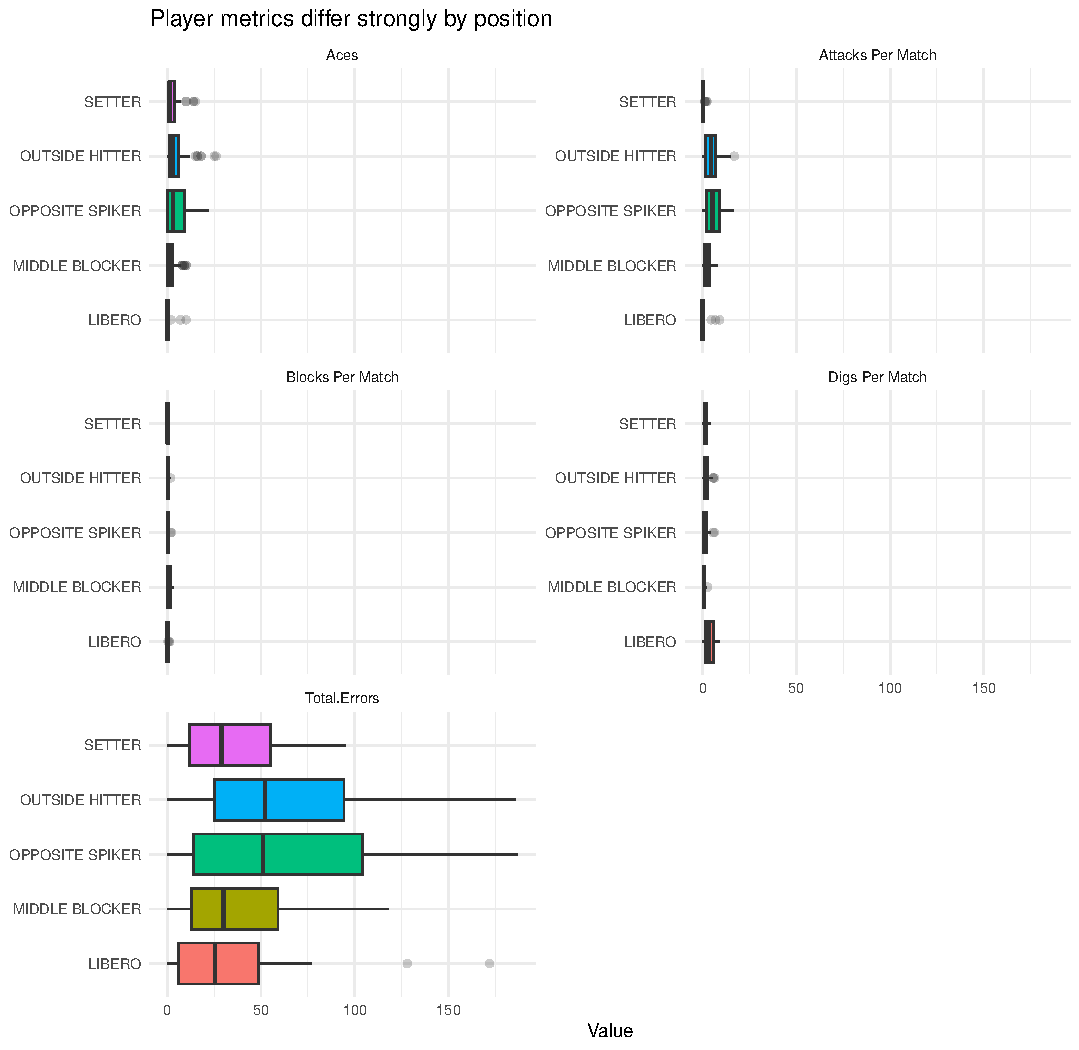
\includegraphics[width=.72\textwidth]{../../outputs/exercise2/position_profiles.pdf}
\caption{Selected player metrics by position. Scales differ between panels.}\label{fig:profiles}\end{figure}

\subsection{Correlations and outliers}
Figure~\ref{fig:corr} shows correlations among demographics, role rates, and total errors. Correlation is interpreted descriptively because position and exposure are common causes; it does not establish that one activity causes errors. In particular, cumulative total errors should rise with opportunities even if error propensity is unchanged.
\begin{figure}[!htbp]\centering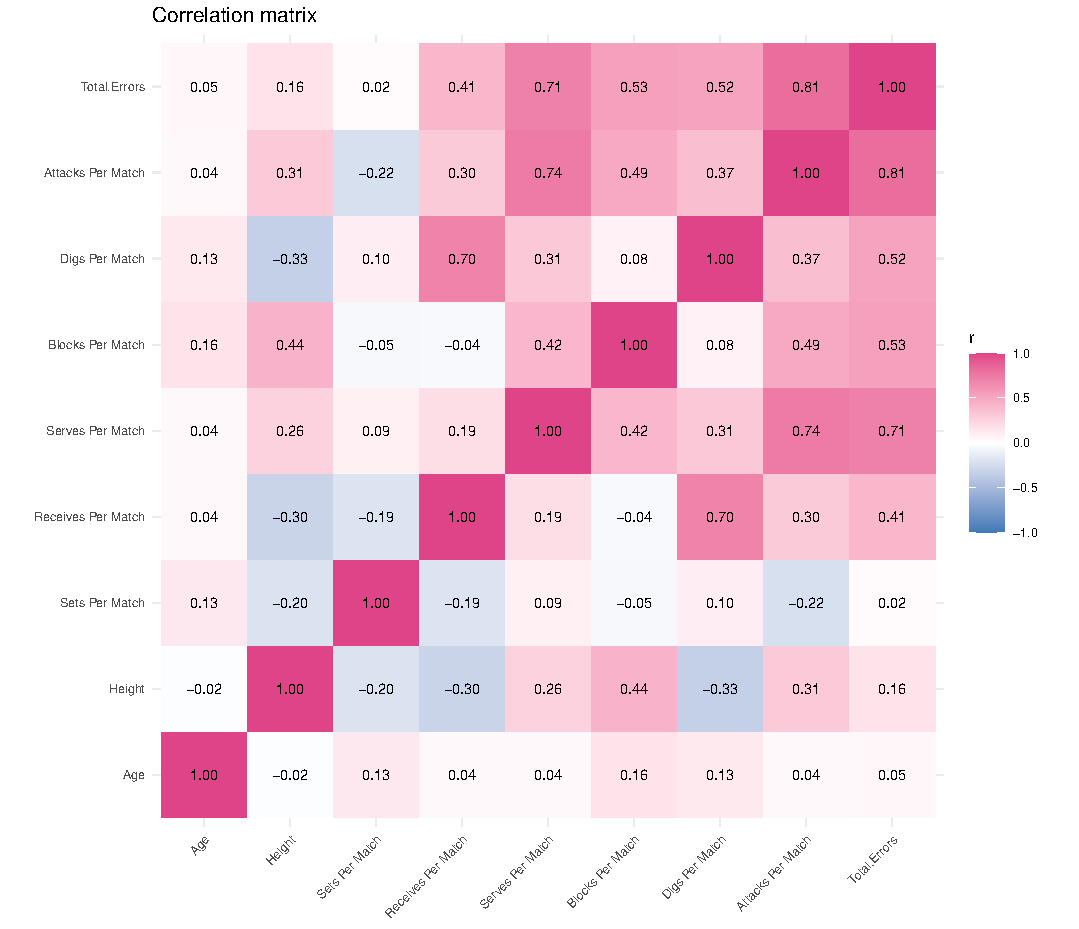
\includegraphics[width=.68\textwidth]{../../outputs/exercise2/correlation_matrix.pdf}
\caption{Pearson correlations for a deliberately non-redundant variable subset.}\label{fig:corr}\end{figure}

Univariate outliers were flagged separately for every numeric variable using Tukey's fences $[Q_1-1.5IQR,Q_3+1.5IQR]$. This distribution-free screen appropriately identifies extremes but does not label them as data errors. The full table records fences and counts. Multivariate outliers were assessed using squared Mahalanobis distances on eight standardised demographic and per-match variables. Distances were calculated within each position so that legitimate role specialisation was not itself labelled anomalous. At the 99\% $\chi^2_8$ cutoff of 20.09, 18 players were flagged: three liberos, seven middle blockers, no opposite spikers, four outside hitters, and four setters. These are unusual profiles for their role, not automatic data errors. Position-conditional calculation is important here: a pooled distance would incorrectly treat legitimate libero and setter profiles as anomalies.

\section{Task 6: Country-level comparison}
All numeric player variables were averaged within the 18 country codes and joined to the supplied team statistics through an explicit code-to-country lookup. Figure~\ref{fig:team} compares player activity with official wins. Mean aces has a moderate positive correlation with wins ($r=.627$), and mean serves per match also correlates positively ($r=.570$). These exploratory associations do not establish that serving alone explains standings; the comparison contains only 18 country-level observations and is sensitive to roster composition. Aggregation also weights every listed player equally rather than by court time, an ecological limitation that prevents player-level causal conclusions.
\begin{figure}[!htbp]\centering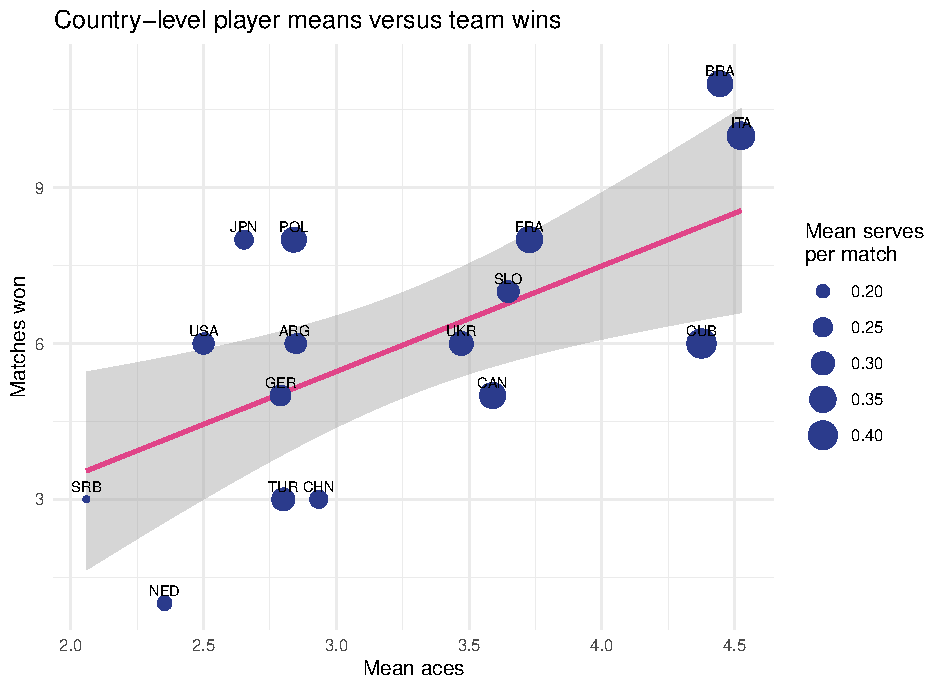
\includegraphics[width=.65\textwidth]{../../outputs/exercise2/team_comparison.pdf}
\caption{Country mean aces against team wins; point size represents mean serves per match.}\label{fig:team}\end{figure}

\section{Task 7: Best and worst by total errors}
For each position, the minimum and maximum requested total were selected, resolving ties alphabetically for reproducibility. The best/worst totals are: libero Alexandre (Brazil, 0) / Ivovi\'{c} (Serbia, 172); middle blocker Ertu\u{g}rul Gazi (T\"urkiye, 0) / Judson (Brazil, 118); opposite Gonzalez (Cuba, 0) / Masso (Cuba, 187); outside hitter Strehlau (France, 0) / Yant (Cuba, 186); and setter Muhammed K. (T\"urkiye, 0) / Giannelli (Italy, 95). The single requested tibble is exported.
\begin{table}[!htbp]
\centering
\small
\begin{tabular}{lrr}
\toprule
Position & Best (errors) & Worst (errors) \\
\midrule
Libero & Alexandre (0) & Ivovi\'{c} (172) \\
Middle blocker & Ertu\u{g}rul Gazi (0) & Judson (118) \\
Opposite spiker & Gonzalez (0) & Masso (187) \\
Outside hitter & Strehlau (0) & Yant (186) \\
Setter & Muhammed K. (0) & Giannelli (95) \\
\bottomrule
\end{tabular}
\caption{Best and worst player within each position under the requested total-error criterion.}
\label{tab:best-worst}
\end{table} Crucially, zero errors may indicate little participation; ``best'' here means only the assignment's total-error criterion, not best performance.

\FloatBarrier
\section{Conclusion}
Position is the dominant organising factor in the player data. Extreme values are frequent but plausible in specialised roles. Country-level serving means show moderate associations with wins, but do not by themselves explain standings. Rate- or exposure-adjusted error measures would support fairer player evaluation.
\section*{Statement of Contributions}
Indudhara Swamy Vivekananda conducted the data preparation, analysis, visualisation, interpretation, and report preparation. This statement must be updated if additional group members contributed.
\end{document}



